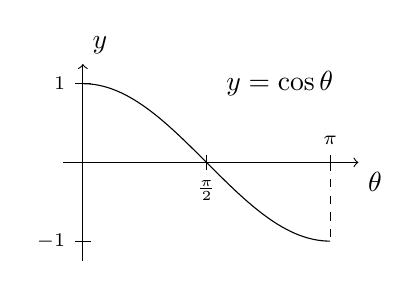
\begin{tikzpicture}
	\draw[->] (-0.25,0) to (3.5,0) node[below right] {$\theta$};
	\draw[->] (0,-1.25) to (0,1.25) node[above right] {$y$};

	\draw[dashed] (3.14,0) to (3.14,-1);
	\draw (0,1) cos (1.57,0) sin (3.14,-1);
	\draw (3.14,-0.1) to (3.14,0.1) node[above] {$\scriptstyle \pi$};

	\draw (1.57,0.1) to (1.57,-0.1) node[below] {$\scriptstyle \frac{\pi}{2}$};
	\foreach \y in {-1,1} {
    \draw (0.1,\y) to (-0.1,\y) node[left] {$\scriptstyle \y$};
  }

	\node at (2.5,1) {$y=\cos\theta$};
\end{tikzpicture}
